\chapter{Réalisation} \label{Chapter4}

\section{Introduction}

\section{Environnement de développement}
Il s’agit dans cette partie d’identifier les différentes caractéristiques de l’environnement matériel et logiciel qui nous ont servi à l’implémentation de notre application.

\subsection{Environnement matériel}
La machine utilisée pour réaliser ce site est un ordinateur portable Lenovo qui a la configuration suivante :

\paragraph{Système d’exploitation} Windows 10
\paragraph{Processeur} Intel(R) Core(TM) i7-8550U CPU
\paragraph{Mémoire RAM installée} 8,00 Go

\subsection{Environnement logiciel}
Nous allons maintenant donner une brève définition de chaque langage et bibliothèque utilisés.

\subsection*{Git}
\begin{wrapfigure}{r}{0.30\textwidth} %this figure will be at the right
    \centering
    
\includegraphics[width=0.2\textwidth]{Figures/git.png}
    \caption{Git}
\end{wrapfigure}
Git est un système de contrôle de version. Il conserve un historique de toutes les modifications apportées au code. Les modifications sont stockées dans une base de données spéciale appelée "repository", également connue sous le nom de "repo".

L'utilisation de Git pour le développement de logiciels présente deux avantages principaux :
\begin{itemize}
    \item Le suivi des modifications et des mises à jour. On est capable de voir qui a fait quels changements. Git permet également de savoir quand et pourquoi un changement a été effectué.
    \item Permettre de travailler en collaboration. Les projets de développement de logiciels nécessitent généralement que de nombreuses personnes travaillent ensemble. Git fournit aux développeurs un moyen systématique de le faire. Ainsi, les développeurs se concentrent sur le projet plutôt que sur les longues sessions de communication entre les autres développeurs.
    \item Il existe d'autres systèmes de contrôle de version, tels que Subversion, Mercurial, etc. Cependant, Git est le plus populaire.
\end{itemize}

Pendant le processus de réalisation, nous utiliserons la plateforme GiHub.

\subsection*{Python}
\begin{wrapfigure}{r}{0.30\textwidth} %this figure will be at the right
    \centering
    
\includegraphics[width=0.15\textwidth]{Figures/python.png}
    \caption{Python}
\end{wrapfigure}
Python est un langage de programmation open-source, interprété, orienté objet, de haut niveau avec une sémantique dynamique, avec des applications dans de nombreux domaines, notamment la programmation web, les scripts, le calcul scientifique et l'intelligence artificielle. Il est bien structuré et nombre de ses fonctionnalités prennent en charge la programmation fonctionnelle, la méta programmation et les méta-objets.

Il est très populaire et largement utilisé par des organisations connues telles que la NASA et Google, entre autres.


\subsection*{La bibliothèque \texttt{mysql-connector-python}}
\begin{wrapfigure}{r}{0.30\textwidth} %this figure will be at the right
    \centering
    
\includegraphics[width=0.20\textwidth]{Figures/mysql.png}
    \caption{mysql-connector-python}
\end{wrapfigure}
MySQL est un système de gestion de bases de données relationnelles (SGBDR) open source et gratuit qui utilise le langage de requête structuré (SQL).
Dans cet article, nous allons partager une explication complète sur MySQL. Il s'agit d'un système de gestion de base de données relationnelle (SGBDR) open-source avec un modèle client-serveur.  Un SGBDR est un logiciel ou un service utilisé pour créer et gérer des bases de données basées sur un modèle relationnel.

Nous avons décidé dans ce projet d'utiliser python au lieu du langage Java, pour la simplicité et la disponibilité de la bibliothèque \texttt{mysql-connector-python}.

\section{Création de la base de données}
\begin{lstlisting}[
    language=SQL,
    showspaces=false,
    basicstyle=\ttfamily,
    numbers=left,
    numberstyle=\tiny,
    commentstyle=\color{gray}
]
--
-- Database : Home
--
DROP DATABASE IF EXISTS Home;
CREATE DATABASE IF NOT EXISTS Home;
USE Home;
\end{lstlisting}

\subsection{Création des tables de la base de données}
\subsubsection*{Utilisateur}
\begin{lstlisting}[
    language=SQL,
    showspaces=false,
    basicstyle=\ttfamily,
    numbers=left,
    numberstyle=\tiny,
    commentstyle=\color{gray}
]
--
-- Structure de la table : utilisateur
--
DROP TABLE IF EXISTS user;
CREATE TABLE IF NOT EXISTS user (
    user_id INT NOT NULL AUTO_INCREMENT,
    user_name VARCHAR(50) NOT NULL,
    user_password VARCHAR(50) NOT NULL,
    user_last_session DATETIME NOT NULL,

    PRIMARY KEY (user_id)
);
\end{lstlisting}

\subsubsection*{Ville}
\begin{lstlisting}[
    language=SQL,
    showspaces=false,
    basicstyle=\ttfamily,
    numbers=left,
    numberstyle=\tiny,
    commentstyle=\color{gray}
]
--
-- Structure de la table : City
--
DROP TABLE IF EXISTS City;
CREATE TABLE IF NOT EXISTS City (
    zip_code INT NOT NULL AUTO_INCREMENT,

    city_name VARCHAR(50) NOT NULL,

    PRIMARY KEY (zip_code)
);
\end{lstlisting}

\subsubsection*{Catégorie}
\begin{lstlisting}[
    language=SQL,
    showspaces=false,
    basicstyle=\ttfamily,
    numbers=left,
    numberstyle=\tiny,
    commentstyle=\color{gray}
]
--
-- Structure de la table : Category
--
DROP TABLE IF EXISTS Category;
CREATE TABLE IF NOT EXISTS Category (
    category_id INT NOT NULL AUTO_INCREMENT,

    category_nom VARCHAR(50) NOT NULL,

    PRIMARY KEY (category_id)
);
\end{lstlisting}

\subsubsection*{Entreprise}
\begin{lstlisting}[
    language=SQL,
    showspaces=false,
    basicstyle=\ttfamily,
    numbers=left,
    numberstyle=\tiny,
    commentstyle=\color{gray}
]
--
-- Structure de la table : Company
--
DROP TABLE IF EXISTS Company;
CREATE TABLE IF NOT EXISTS Company (
    company_id INT NOT NULL AUTO_INCREMENT,

    product_id INT NOT NULL,

    company_name VARCHAR(50) NOT NULL,
    company_email VARCHAR(50) NOT NULL,
    company_description VARCHAR(50) NOT NULL,

    PRIMARY KEY (company_id),
    FOREIGN KEY (product_id) REFERENCES Product(product_id)
);
\end{lstlisting}

\subsubsection*{Contrôle}
\begin{lstlisting}[
    language=SQL,
    showspaces=false,
    basicstyle=\ttfamily,
    numbers=left,
    numberstyle=\tiny,
    commentstyle=\color{gray}
]
--
-- Structure de la table : Control
--
DROP TABLE IF EXISTS Control;
CREATE TABLE IF NOT EXISTS Control (
    control_id INT NOT NULL AUTO_INCREMENT,

    stock_id INT NOT NULL,

    control_date DATETIME NOT NULL,

    PRIMARY KEY (control_id),
    FOREIGN KEY (stock_id) REFERENCES Stock(stock_id)
);
\end{lstlisting}

\subsubsection*{Stock}
\begin{lstlisting}[
    language=SQL,
    showspaces=false,
    basicstyle=\ttfamily,
    numbers=left,
    numberstyle=\tiny,
    commentstyle=\color{gray}
]
--
-- Structure de la table : Stock
--
DROP TABLE IF EXISTS Stock;
CREATE TABLE IF NOT EXISTS Stock (
    stock_id INT NOT NULL AUTO_INCREMENT,

    product_id INT NOT NULL,

    stock_name VARCHAR(50) NOT NULL,

    PRIMARY KEY (stock_id),
    FOREIGN KEY (product_id) REFERENCES Product(product_id)
);
\end{lstlisting}

\subsubsection*{Information}
\begin{lstlisting}[
    language=SQL,
    showspaces=false,
    basicstyle=\ttfamily,
    numbers=left,
    numberstyle=\tiny,
    commentstyle=\color{gray}
]
--
-- Structure de la table : Information
--
DROP TABLE IF EXISTS Information;
CREATE TABLE IF NOT EXISTS Information (
    information_id INT NOT NULL AUTO_INCREMENT,

    information_expiration_date DATETIME NOT NULL,
    information_entry_date DATETIME NOT NULL,
    information_unit_price INT NOT NULL,
    information_quantity INT NOT NULL,

    PRIMARY KEY (information_id)
);
\end{lstlisting}

\subsubsection*{Taille}
\begin{lstlisting}[
    language=SQL,
    showspaces=false,
    basicstyle=\ttfamily,
    numbers=left,
    numberstyle=\tiny,
    commentstyle=\color{gray}
]
--
-- Structure de la table : Shape
--
DROP TABLE IF EXISTS Shape;
CREATE TABLE IF NOT EXISTS Shape (
    shape_id INT NOT NULL AUTO_INCREMENT,

    shape_name VARCHAR(50) NOT NULL,
    shape_height VARCHAR(50) NOT NULL,
    shape_weight VARCHAR(50) NOT NULL,
    shape_volume VARCHAR(50) NOT NULL,

    PRIMARY KEY (shape_id)
);
\end{lstlisting}

\subsubsection*{Produit}
\begin{lstlisting}[
    language=SQL,
    showspaces=false,
    basicstyle=\ttfamily,
    numbers=left,
    numberstyle=\tiny,
    commentstyle=\color{gray}
]
--
-- Structure de la table : Product
--
DROP TABLE IF EXISTS Product;
CREATE TABLE IF NOT EXISTS Product (
    product_id INT NOT NULL AUTO_INCREMENT,

    shape_id INT NOT NULL,
    information_id INT NOT NULL,
    category_id INT NOT NULL,

    product_name VARCHAR(50) NOT NULL,
    product_temperature_max VARCHAR(50) NOT NULL,
    product_temperature_min VARCHAR(50) NOT NULL,
    product_description VARCHAR(50) NOT NULL,

    PRIMARY KEY (product_id),
    FOREIGN KEY (shape_id) REFERENCES Shape(shape_id),
    FOREIGN KEY (information_id) REFERENCES Information(information_id),
    FOREIGN KEY (category_id) REFERENCES Category(category_id)
);
\end{lstlisting}

\subsubsection*{Appartenir}
\begin{lstlisting}[
    language=SQL,
    showspaces=false,
    basicstyle=\ttfamily,
    numbers=left,
    numberstyle=\tiny,
    commentstyle=\color{gray}
]
--
-- Structure de la table : BELONGING
--
DROP TABLE IF EXISTS BELONGING;
CREATE TABLE IF NOT EXISTS BELONGING (
    zip_code INT NOT NULL,
    company_id INT NOT NULL,

    FOREIGN KEY (zip_code) REFERENCES City(zip_code),
    FOREIGN KEY (company_id) REFERENCES Company(company_id),
    CONSTRAINT PRIMARY KEY (
        zip_code,
        company_id
    )
);
\end{lstlisting}

\subsection{Contraintes d'intégrité}
\begin{lstlisting}[
    language=SQL,
    showspaces=false,
    basicstyle=\ttfamily,
    numbers=left,
    numberstyle=\tiny,
    commentstyle=\color{gray}
]
--
-- Contraintes d'intégrité
--

ALTER TABLE Product
ADD CONSTRAINT
    CHECK (
        product_temperature_max > 0 AND
        product_temperature_min > 0
    );

ALTER TABLE Shape
ADD CONSTRAINT
    CHECK (
        shape_height > 0 AND
        shape_weight > 0 AND
        shape_volume > 0 AND
    );

ALTER TABLE Information
ADD CONSTRAINT
    CHECK (
        information_quantity > 0 AND
        information_entry_date <= information_expiration_date AND
        information_unit_price > 0
    );

ALTER TABLE Control
MODIFY control_results ENUM (
    'Produit est périmé',
    'Produit est disponible',
    'Produit n est pas disponile'
);
\end{lstlisting}

\subsection{Commandes SQL}
Cette partie a pour objectif : tester toutes les requêtes avant de les ajouter dans le code permettant de contrôler l’application.

\subsubsection{Requêtes concernant l'affichage d'un produit}
\begin{lstlisting}[
    language=SQL,
    showspaces=false,
    basicstyle=\ttfamily,
    numbers=left,
    numberstyle=\tiny,
    commentstyle=\color{gray}
]
SELECT product_name, category_name
FROM Product, Category
WHERE Product.category_id = Category.category_id;
\end{lstlisting}


\subsubsection{Requêtes concernant l'affichage de derniers résultats de contrôle des produits}
\begin{lstlisting}[
    language=SQL,
    showspaces=false,
    basicstyle=\ttfamily,
    numbers=left,
    numberstyle=\tiny,
    commentstyle=\color{gray}
]
SELECT product_name, control_results
FROM Product, Control, Stock
Where
	Control.stock_id = Stock.stock_id AND
    Stock.product_id = Product.product_id
GROUP by product_name;
\end{lstlisting}


\subsubsection{Requêtes concernant modification de mot de passe}
\begin{lstlisting}[
    language=SQL,
    showspaces=false,
    basicstyle=\ttfamily,
    numbers=left,
    numberstyle=\tiny,
    commentstyle=\color{gray}
]
UPDATE User
SET
    user_password = password
WHERE
    user_name = name;
\end{lstlisting}

\subsubsection{Requêtes concernant la suppression d'un produit}
\begin{lstlisting}[
    language=SQL,
    showspaces=false,
    basicstyle=\ttfamily,
    numbers=left,
    numberstyle=\tiny,
    commentstyle=\color{gray}
]
DELETE FROM User
WHERE product_name = name
\end{lstlisting}

\section{Interfaces}

\begin{figure}[ht!]
    \centering
    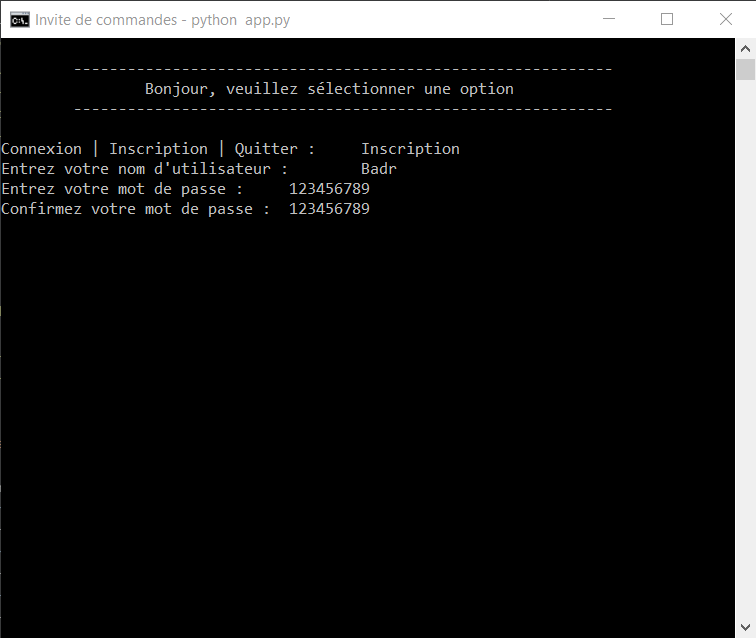
\includegraphics[keepaspectratio=true,scale=0.7]{Figures/img1.png}
    \caption{Ouvrir un compte}
    \label{fig:img1}
\end{figure}

\begin{figure}[ht!]
    \centering
    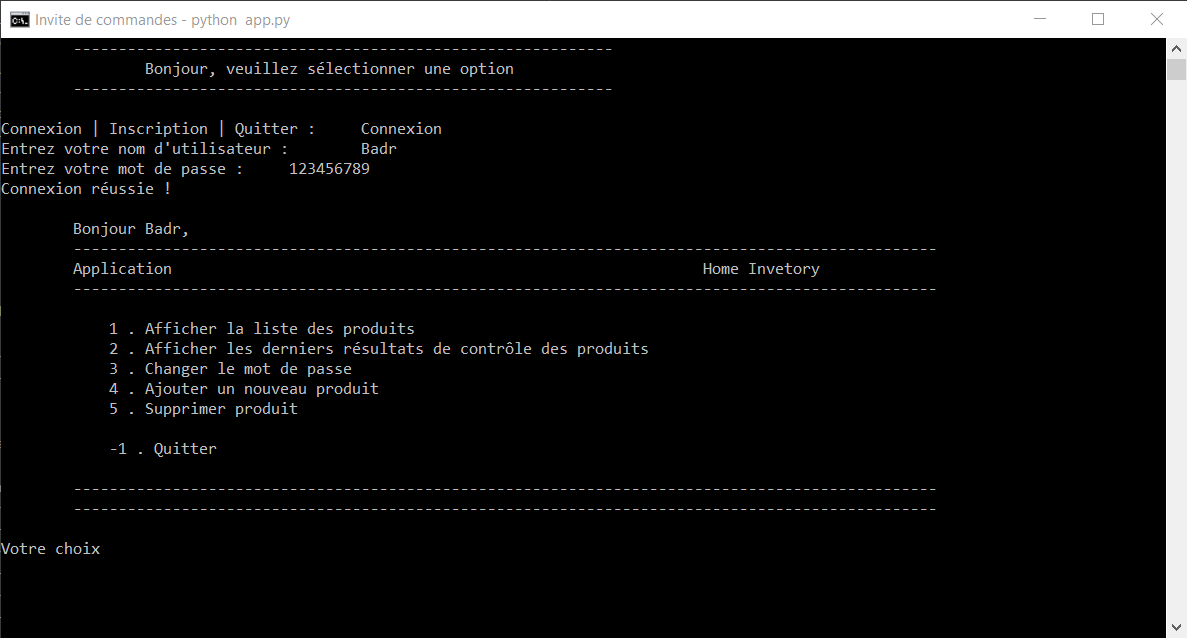
\includegraphics[keepaspectratio=true,scale=0.7]{Figures/img2.png}
    \caption{Page d'accueil}
    \label{fig:img1}
\end{figure}

\begin{figure}[ht!]
    \centering
    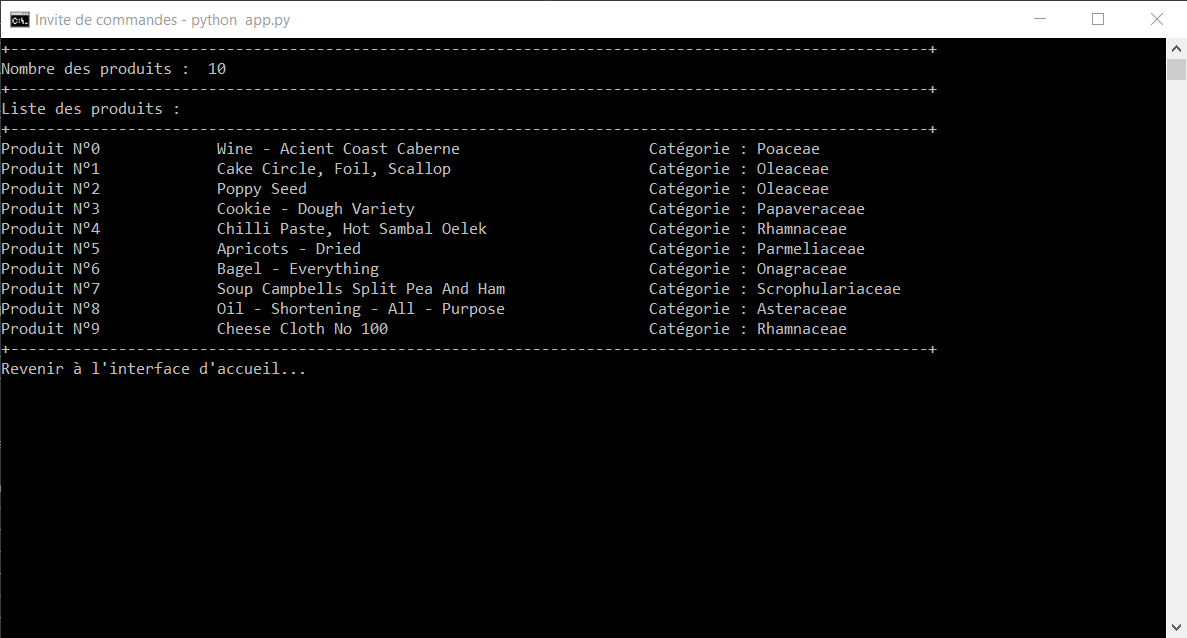
\includegraphics[keepaspectratio=true,scale=0.7]{Figures/img3.png}
    \caption{Liste des produits}
    \label{fig:img1}
\end{figure}

\begin{figure}[ht!]
    \centering
    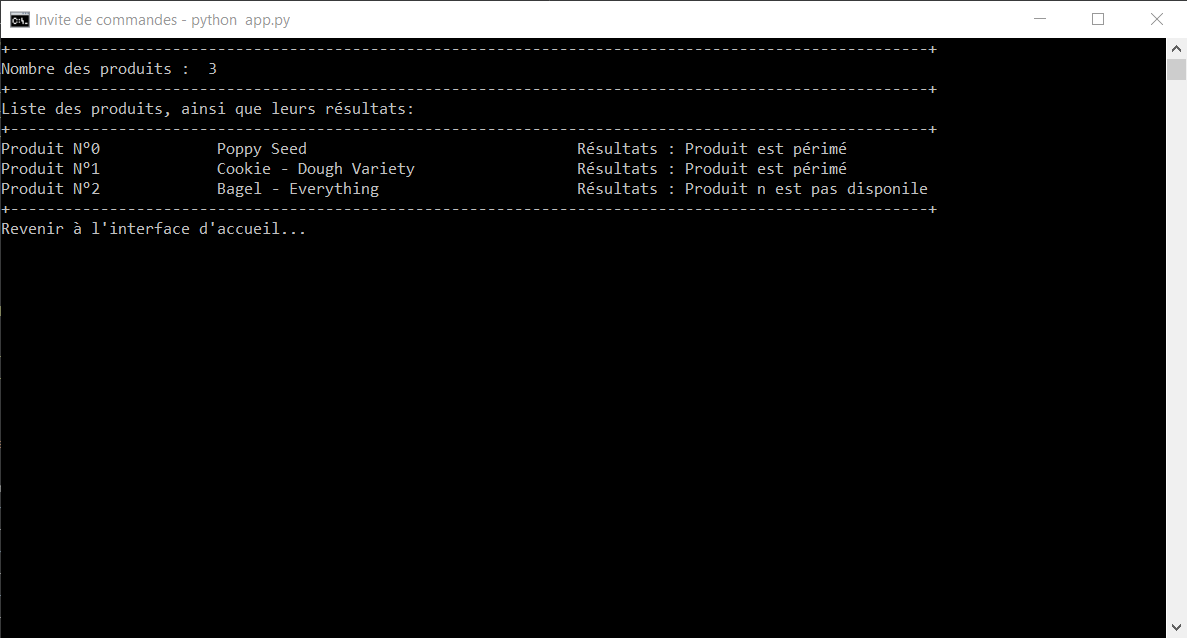
\includegraphics[keepaspectratio=true,scale=0.7]{Figures/img4.png}
    \caption{Liste des résultats de contrôle}
    \label{fig:img1}
\end{figure}
